\documentclass{article}

% Appearance
%--------------------------------------
\usepackage[a4paper,width=170mm,top=18mm,bottom=22mm,includeheadfoot,marginparsep=2cm]{geometry}
\usepackage{url}
\usepackage{enumitem}
%--------------------------------------

% Colors
%--------------------------------------
\usepackage{color}
\definecolor{lightyellow}{rgb}{1,0.98,0.9}
%--------------------------------------

% Language
%--------------------------------------
\usepackage[utf8]{inputenc}
\usepackage[T2A]{fontenc}
\usepackage{hyphenat}
\hyphenation{he-lio-trope opos-sum}
\usepackage{csquotes}
%--------------------------------------

% References
%--------------------------------------
\usepackage{biblatex}
\addbibresource{biblio.bib}
%--------------------------------------

% Footnotes
%--------------------------------------
\usepackage[hang]{footmisc}
\setlength{\footnotemargin}{14pt}
\setlength{\skip\footins}{20pt}
%--------------------------------------

% Columns
%--------------------------------------
\usepackage{multicol}
\setlength{\columnsep}{24pt}
%--------------------------------------

% Graphics
%--------------------------------------
\usepackage{graphicx}
\graphicspath{{images/}}
%--------------------------------------

% Tables
%--------------------------------------
\usepackage{array, tabularx, caption, boldline}
\usepackage{graphicx}
\usepackage{cellspace}
\usepackage{makecell}
\renewcommand\theadfont{\normalfont\bfseries}
\def\arraystretch{2}
%--------------------------------------

% Math
%--------------------------------------
\usepackage{amsmath}
%--------------------------------------

\title{BankEx Proof-of-Asset Protocol}
\author{Yellow Paper, version 0.1.4 alpha}
\date{September 03, 2017}

\begin{document}

\pagecolor{lightyellow}

\maketitle

\begin{abstract}
BankEx Proof-of-Asset protocol of assets tokenization and liquidity increase is being described. Practical implementation of the Proof-of-Asset Protocol based on Ethereum platform smart-contracts is being described enlightening technical and economical aspects of the protocol.
\end{abstract}

\vspace{24pt}

\begin{multicols}{2}

\tableofcontents

\section{Introduction}

\subsection{BankEx Proof-of-Asset Protocol}

BankEx is an organization that unites members of the financial markets in order to build a community and implement the Proof-of-Asset Protocol enables community members to profit from mutual use of assets. 

The product of BankEx is the Proof-of-Asset Protocol, which solves the issue of non-fungible asset liquidity. Proof-of-Asset means the token released as part of the protocol is ensured with an asset. 
The know-how of BankEx is the Proof-of-Asset protocol, in essence a combination of BaaS (Bank-as-a-Service) and blockchain technologies. We take a client asset, primarily on the financial market, we tokenize it, then, without waiting for the portfolio to accumulate critical mass, we turn this asset into money for the bank.  This is made possible through formation of a single pool of similar assets (e.g., pool of banks) thereby creating a marketplace, where banks benefit from liquidity and investors benefit from a predictable and transparent cash flow.

\subsection{Specification of Examples in Yellow Paper}

All examples and demonstrations in this Yellow Paper are used only as demonstrative examples of the SmartDeal technology. The business of BankEx involves manufacturing fintech products and tokenizing primarily financial assets, although we do not think it impossible to apply the Proof-of-Asset Protocol in other fields, with approval from the BankEx Foundation in case of non-financial Smart Assets. In our case, first and foremost we create liquidity for financial assets.

\subsection{Game Theory Behind the Proof-of-Asset Protocol}

Game Theory\footnote{\textbf{Game theory} is the study of the ways in which \textit{interacting choices} of \textit{economic agents} produce outcomes with respect to the \textit{preferences} (or \textit{utilities}) of those agents, where the outcomes in question might have been intended by none of the agents \cite{stanfordGameTheory}.} is a branch of mathematical economics focusing on the outcomes of conflicts between players, and the optimality of their strategies. Analysis carried out according to game theory indicates that the global financial market is currently trapped in the sub-optimal equilibrium of the prisoner’s dilemma. This dilemma is a fundamental problem of game theory, illustrating how players will sometimes fail to cooperate even if it was in their best interest.

We see that players in financial markets distrust each other and keep overpaying for an inefficient set of various ratings, scores and audits, although these are frequently wrong (as with the Enron scandal and the subprime mortgage crisis). This inefficiency leads to high costs and often losses, which in turn raise the cost of capital and lead to a lack of access to capital for decentralized small businesses or borrowers. Another issue derived from this dilemma is the obstructing cost of deployment to the public market. If this barrier is removed, then the market itself is cable to evaluate every asset based on the collective wisdom of all trading participants, as the increase in volume of transparent and authentic trade operations provides more information that can be used by the market to verify the assets.

We offer a solution~--- the Proof-of-Asset Protocol, the point of which is an instant audit of the asset. Now every investor is aware of the status of his investments in non-public companies and assets. Equipped with this tool, the market will force certain businesses to change (lawyers, accounting, auditors, and in separate cases banks and collectors). What is our plan? We will begin by modernizing the mechanisms of assigning and validating ratings, as the cash flow recorded on the blockchain using the Proof-of-Asset protocol is transparent, understandable, as well as much faster and cheaper. In essence, the asset’s state is being constantly monitored by the logic of smart-contracts.  

In turn, the increased amount of information on economical operations and their authenticity grant new opportunities for the development of an economical AI, building sufficiently precise artificial intelligence systems for risk evaluation, making the cost of such calculations approach zero. This would enable the creation of a competitive market of economical AI working for the good of modern society. 

\section{Modern Financial Markets}

\subsection{Classical Microservice Architecture}

Microservice architecture is a network of module services that can be deployed independently from one another.

Microservice architecture is an approach to structuring applications whereby they are broken down into smaller independent internal components.

\paragraph{Advantages of Microservice Architecture:}

\begin{itemize}
\item autonomous ownership for different microservices within an application;
\item agility, application micro-components can be developed and tested in autonomous decentralized teams much faster;
\item improved scalability (scaling independent of other components, on-demand scaling);
\item continuous delivery and deployment of micro-components.
\end{itemize}

A monolithic architecture is much easier in implementation, control and deployment, while microservices require careful management, as they are deployed on different servers and use API.

Such architecture allows technically complicated applications to constantly evolve without the need to wait for the release of a new version of the product to make changes. There is no need to release an updated version of the product, if the changes apply only to a small part of the product. That’s why it’s possible to customize for various business tasks of every enterprise, department or person.

Notably, microservices can be fully managed by different teams in compliance with different standards and are also more available: even if one of them crashes, it does not lead to the crash of the entire application. A unified architecture facilitates work in situations where multiple modules need to interact with one another, or where classes need to be transferred from one module to another. At the same time microservices can guarantee that there will be no shared states between the modules. Finally, microservices allow you to use multiple technologies and languages, depending on business needs (Figure~\ref{fig:microservice-vs-monolyth}).

\begin{figure*}
  \centering
  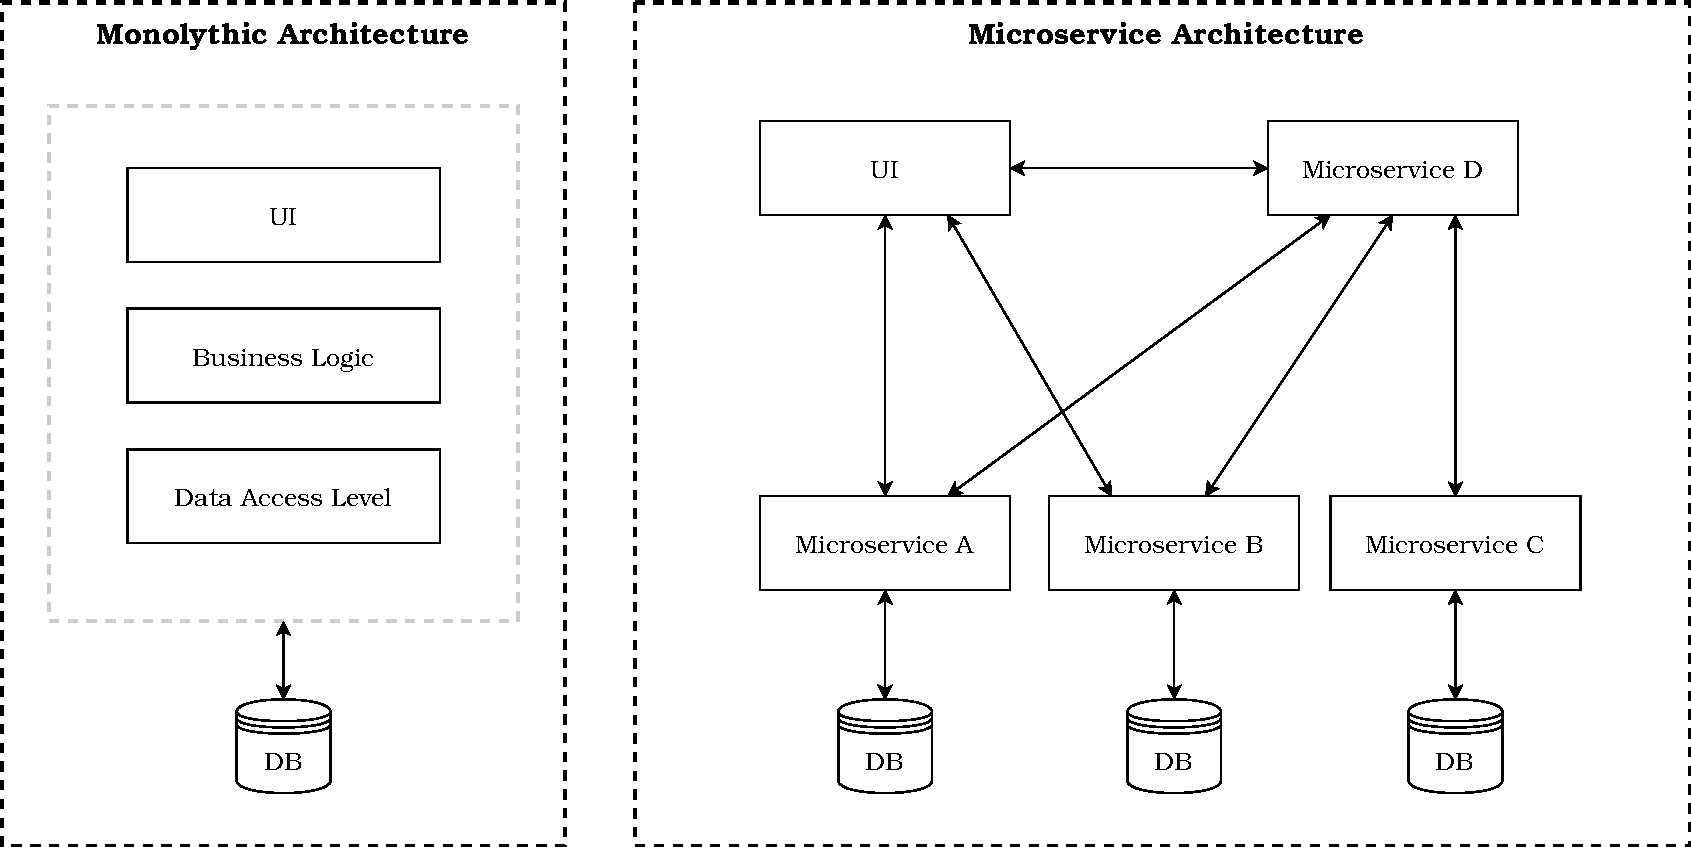
\includegraphics[width=\textwidth]{microservice-vs-monolyth.pdf}
  \caption{Monolythic vs. Microservice Architecture}
  \label{fig:microservice-vs-monolyth}
\end{figure*}

\subsection{Bank-as-a-Service (\textit{BaaS}) Business Model}

Bank-as-a-Service (\textit{BaaS}) is a business model that makes it possible to build new financial products that are integrated with multiple existing technological solutions and jurisdictions. 

On one side of these platforms are originators in various jurisdictions with various technologies, and on the other are fintech-companies wishing to launch a new product or expand to a new market. Thanks to the platform, they are able to do this quickly and efficiently, without the need to work out integration with the legislation of every country and every new bank from scratch. Since the platform already contains technological and legal integration, it can provide access to a new player more cheaply and more quickly. 

\textbf{The originator in the BaaS model} is a storefront, essentially establishing access to the end client, be it a bank, a fintech company, an internet platform, a stock exchange or an insurer. It is critical that when building the BaaS business model, the originator of the platform maintains his client and access to the client under his control, but at the same time he provides the client with the most up-to-date and competitive products on the market by the best tech (fintech, IT) companies on the market. It’s an excellent solution to preserve and monetize clients.

How does an end client see it? Like a bank~--- he does not have to see the third party provider.

There exist several levels of integration of participants of the BaaS model: from primitive analogue integration, where an employee would have to re-enter data into a separate service, to fully automated integration. The originator makes the choice of whichever model of work with an end client is most beneficial to him, either where the end client is shown that the company he is interacting with provides services by outside service providers, or where the end client sees the entire product line under the originator’s brand.

Some researchers call this conception \enquote{The Lego Bank} which owns no pieces but assembles the pieces into different form factors.  The constituent pieces are all the same.  It is how you put the pieces together that makes the difference.  Like Lego, you can build the pieces into a Castle, a House or a Winnebago.  It’s all about how you click pieces together \cite{skinner2017baas}.

As a result, the Bank-as-a-Service platform is a unified window, where corporate or retail clients can choose and receive services that are being offered by various banks and tech companies in various countries. This platform takes over technical and legal integration of various players on the financial market.

\subsection{Decentralized BaaS Model}

According to McKinsey \& Co., there are three main trends in banking evolution:

\begin{itemize}
\item automation;
\item increased regulation;
\item increased pace of technological development.
\end{itemize}

Blockchain allows to automate different processes and banks can benefit from it a lot. Accounting, legal and risk parts might be automated. McKinsey \& Co. states that blockchain, based on advanced cryptography, might allow doing such operations in the most effective, safe and transparent way in human history.

\textbf{For global players, adaptation to such trends will become a vital issue}. Enhanced financial regulation will force participants  to use partner BaaS platforms as adaptation to new jurisdictions independently will become prohibitively expensive. Fast tech development,  which many of the banks can’t handle, will drive banks interest in using other fintech companies’ services. It will drive a demand for BaaS usage.

\textbf{Decentralized BaaS is the future of banking. Why?} The world has changed and financial streams are becoming global. They are no longer easily controlled by common tools. Regulators and central banks, defining the movement of the market, are responding to this with more strict regulations. In turn, banks respond by creating as many service offerings as permitted by their license beyond their confines. They aim to create innovative services, leaving only themselves with just the core.

This trend creates the risk of a bank evolving into something more similar to a telecommunication company~--- a company with a license that no longer sees its clients.

At BankEx we see this risk, but believe it is right for banks to preserve the status of the most important key element of the world’s financial ecosystem. Fintech and IT companies should not be disrupters of the banking system. Instead they should supplement each other in a mutually beneficial way.

Several years ago, banks and innovative technologies existed separately, with banks expressing an interest in external IT products such as certain separate features. Today the market has changed, leading banks of the world work more and more closely with fintech companies, while the fintech companies in turn ceased to see themselves as disruptors triumphing over banks and instead view themselves as partners to banks. Everyone acknowledges that offline bank departments will remain, even if nobody goes to them, as foundations of faith in the system. A customer must understand that the financial service he receives is that of a bank, the bank actually exists, it has a department in the city, to which the customer can go in case of an issue for assistance. This reason at least will remain. This isn’t just a domain that might close tomorrow and leave its end client alone with their issue. On the other hand, fintech and blockchain companies acknowledge that the market share occupied by their products is too small, below 10\%, and in order to amplify it, they must partner with banks.

In other words, fintech products must end up at banks. Clients, in turn, will purchase and use innovative financial products much more willingly if they can do so under the brand of a familiar bank. It’s worth noting that some banks will remain skeptical about integration with fintech companies. Luckily, the banking community understands that fighting innovation will only result in market share loss.

On the other hand, FinTech innovation alone is not sufficient to absorb the exorbitant transaction flows and and vast financial streams. One explanation is that banks don’t trust one another and they don’t trust technological companies. They are afraid of losing their client-base by partnering with a stronger or more technologically advanced player. They are concerned that upon close examination their products will not be competitive compared to alternatives. They are afraid regulators would penalize them for use of innovations in their base products. Another important note is that decisions regarding such risks are made by top-managers, most of whom are more concerned with protecting their reputation than introducing innovation.

Technological progress has presented us with solutions to such issues~--- organizing mutual trust of participants in the system and trust in operations in the system based on decentralized data storage and automated smart-contracts.

Many professional market players admit that a decentralized BaaS business-model is an optimal path to collaboration between classic banks and financial companies with cutting edge IT companies and continually growing decentralized technological companies of the future.

Front service of clients remains in the hands of the banks, while products are presented by narrowly-oriented product banks or companies. 

We believe that the \textit{B2B2C} combination of business-models and technologies is the key to BankEx’s success.

\subsection{Blockchain Serviсe Architecture (\textit{Blockchain~SA})}

On an Ethereum blockchain micro-service, architecture is used in the implementation of external oracles. At the same time, the Ethereum network is itself an example of network that uses the concept of micro-services, since it contains all the characteristic features of micro-services
(Figure~\ref{fig:blockchain-microservice-architecture}):

\begin{itemize}
\item excess and reservation, as each node of the network is autonomous;
\item service discovery for automatic configuration of network topology;
\item extensibility through the use of other types of micro-services (such as oracles, micro-services allowing to display statistics, etc.).
\end{itemize}

\begin{figure*}
  \centering
  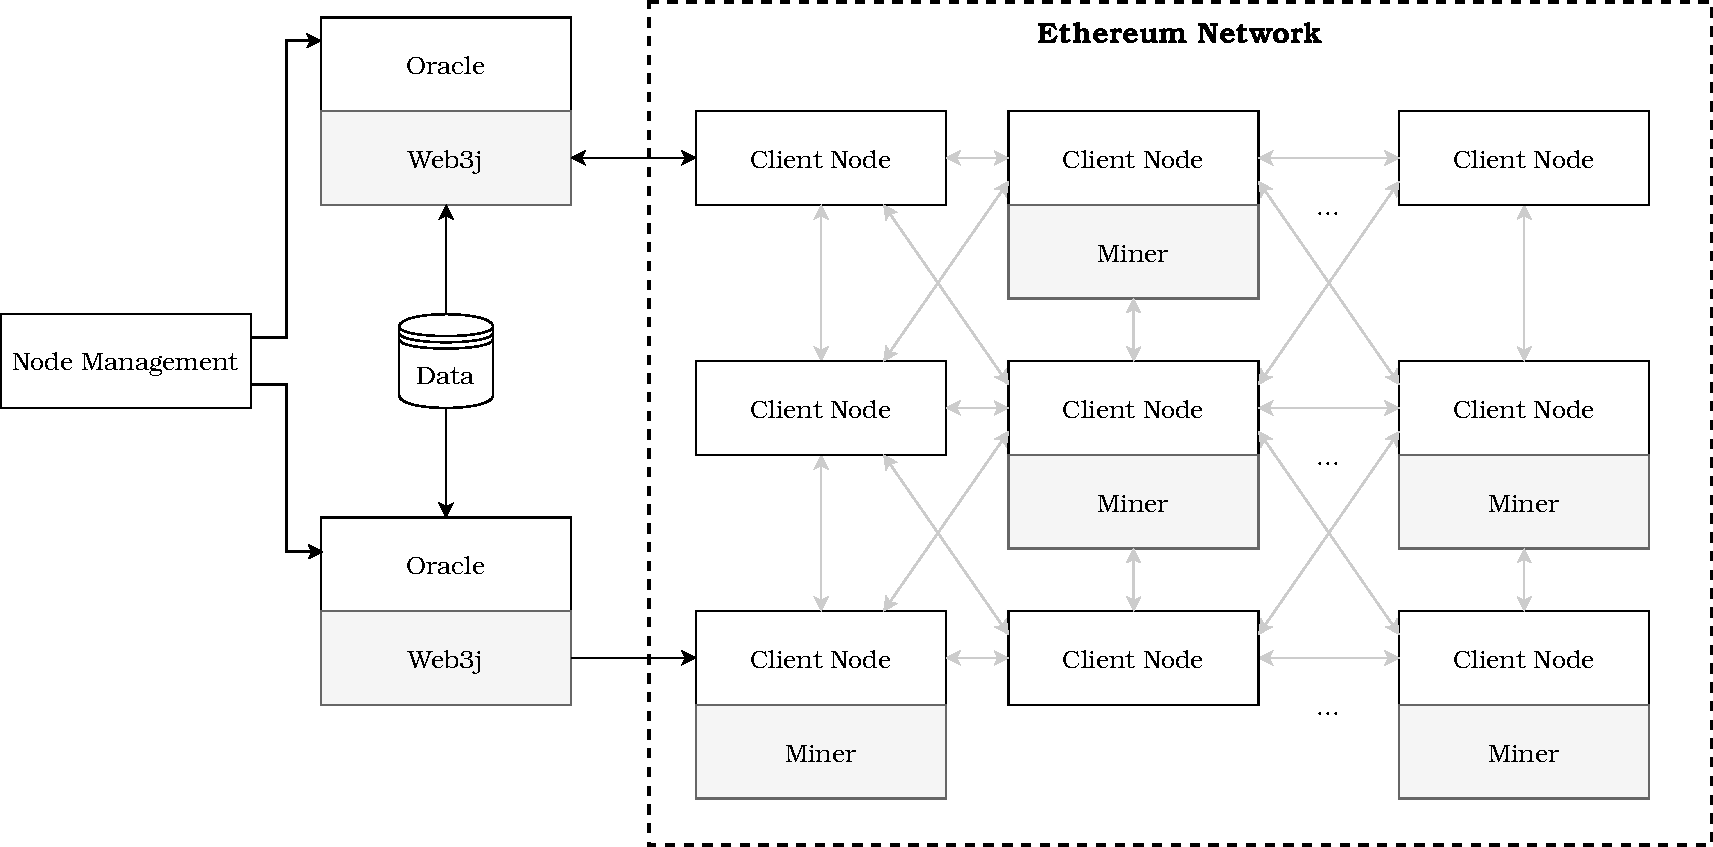
\includegraphics[width=\textwidth]{blockchain-microservice-architecture.pdf}
  \caption{Blockchain Microservice Architecture}
  \label{fig:blockchain-microservice-architecture}
\end{figure*}

The logic of the BankEx liquidity protocol is based on the concept of the Ethereum smart contract\footnote{The phrase \enquote{\textit{smart contract}} was coined by Nick Szabo initially in \cite{szabo1996} and later in \cite{szabo1997}.}, and accordingly uses all of its infrastructure advantages. At the same time, technically, the BankEx protocol is a series of smart contract updates, however these smart contract updates are not micro-services themselves, the micro-services are in relation between API calls themselves. From our side, the business tasks of the protocol, which require a classical micro-service architecture, are realized through the creation of the oracle system. Protocol oracles are designed strictly according to the principles of the micro-services, that is, the instances of these oracles should be automatically added under the required conditions. In this case, dynamic balancing of the number of oracle instances is used. Part of the BankEx oracles is implemented on the basis of Microsoft Azure cloud technologies, since it's one of the most bank friendly platforms. An example of the protocol logic was realized through the interaction with the signals from Internet of Things sensors.

But for the description of the BankEx Proof-of-Asset protocol the definition of the micro-service architecture is not entirely correct. BankEx team calls it the \textit{Blockchain Service Architecture} (\textit{Blockchain~SA}).

\paragraph*{Blockchain~SA} is a sequence of smart contracts, every step of which can be customized by a predetermined pool of actors validated for the particular step of the included smart contracts, while the contents of contracts in a step and the number of steps are embedded in the business logic necessary to tokenize the Smart Asset.

It is an asset tokenization constructor, but one that only works in a sequence of smart contracts correctly arranged after one another, supplemented with oracles connected as micro-services. 

This allows to tokenize an asset with maximum precision and transparency for all participants of the market, while also working in line with the open source BankEx Proof-Of-Asset protocol. 

\subsection{Complexity regulation of the Blockchain~SA}

We often hear from technical experts: Your protocol is too complicated. Other technical gurus say~--- your protocol is too simple. Yes, they are correct. The complexity of the BankEx protocol, which is based on the Blockchain Service Architecture, is regulated by the increase/decrease in the number of smart contracts in the tokenization logic (Figure~\ref{fig:smart-asset-contract-chain}).

\begin{figure*}
  \centering
  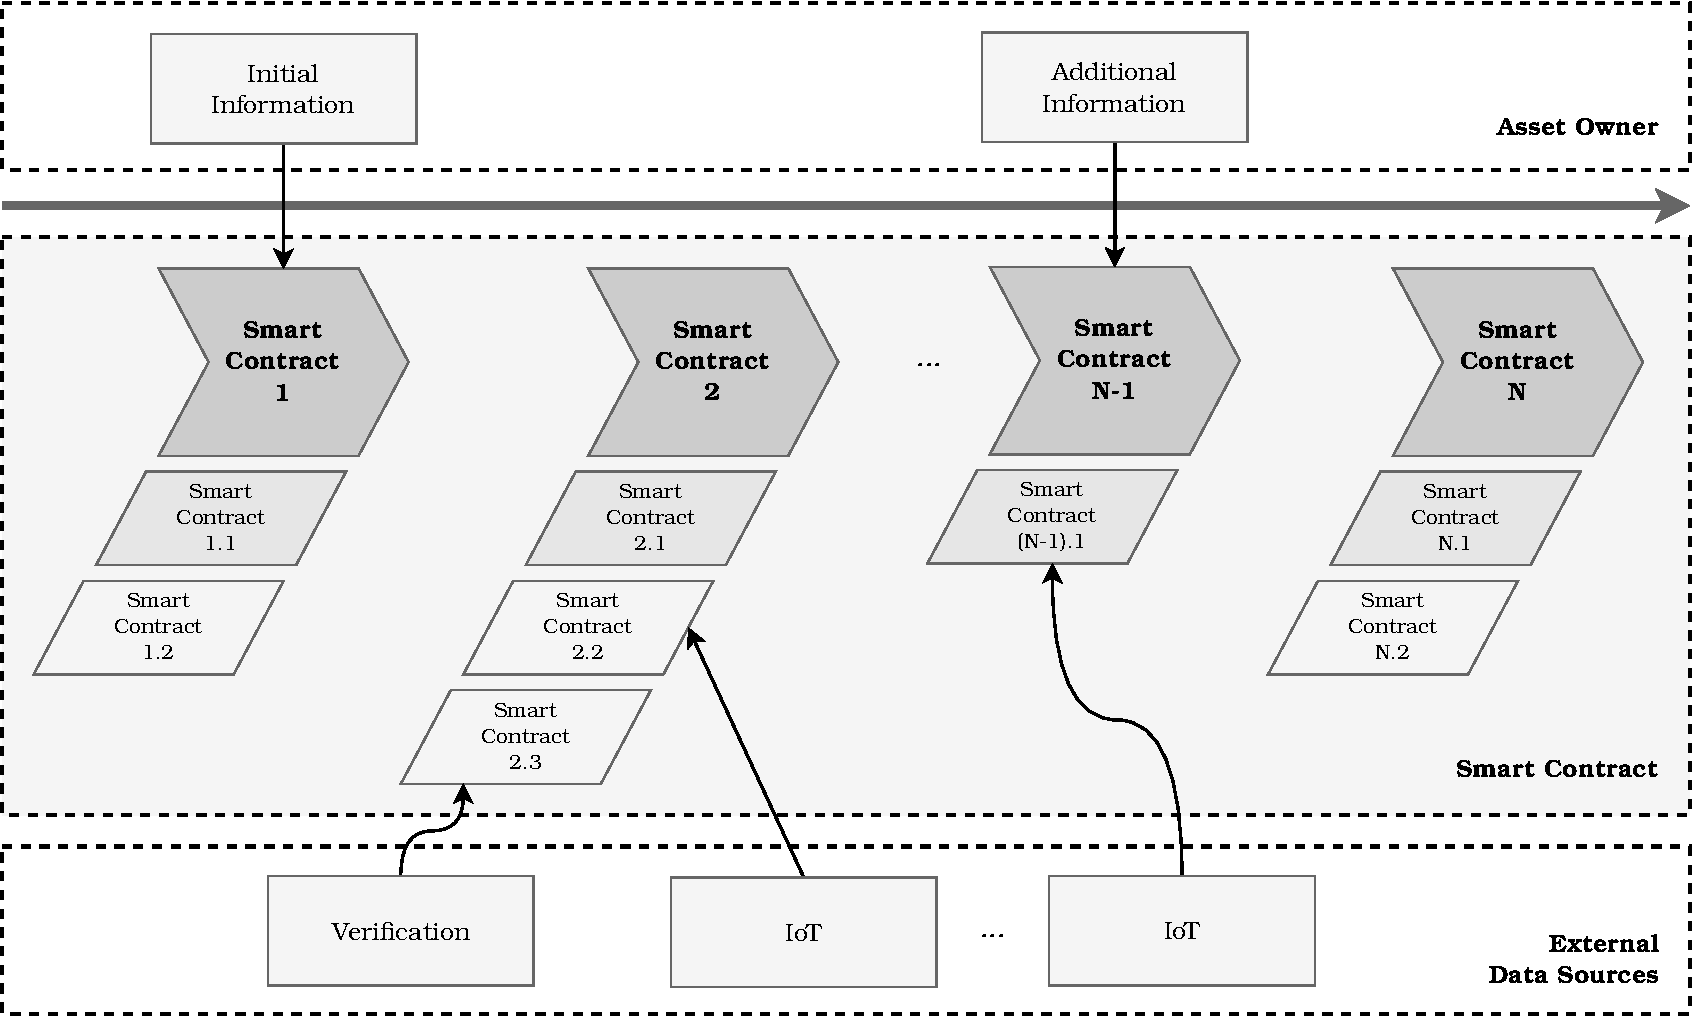
\includegraphics[width=\textwidth]{smart-asset-contract-chain.pdf}
  \caption{Blockchain~SA Smart Contract Chain}
  \label{fig:smart-asset-contract-chain}
\end{figure*}

The creation of a smart asset of a certain type does not necessary use all the steps that are laid out in the Blockchain~SA, only the steps of the smart contract chain that are required by a particular Smart Asset are used. The simplest Smart Asset consists of three steps: initialization, validation, and valuation. And in this case the Smart Asset will fulfill its mission~--- make the asset liquid. It’s not complicated at all. 

At the same time, BankEx is an old company in the sphere of financial technologies, classic fintech. We know very well how complex financial tools can be, and how difficult it is to properly formalize them. Our solution is the Blockchain Service Architecture~--- exactly what you need. You can add any level of complexity to the asset tokenization chain which will result in a Smart Asset.

Moreover, the Smart Asset retains all the features of a blockchain Smart Contract~--- everyone is able to see what value is behind it and how truthful it is. 

You can add your own logic block to the BlockchainService chain~--- Proof-of-Asset Protocol, because it is an open source code. To do that~--- you will need to address the BankEx Foundation community.

\subsection{Benefits of Blockchain~SA}

\paragraph*{Why would the service architecture of the future use blockchain?} In the existing infrastructure, a large application or product consists of a large number of modules which are almost always developed by different teams, and, even if the teams work within the same bank, they still requires a large number of cash flows between different participants in the system and a large amount of agreements and inspections. It is costly, time consuming, and very likely to result in mistakes, including system errors.

Blockchain helps automate the chain of transactions, increasing reliability, transaction transparency and removing inefficiencies and bureaucratic hurdles. It lowers the risk of human mistakes and for many operations completely removes the need for human intervention. This will make your business faster, lower your costs and increase the market's trust in you.

Finally, Blockchain Service Architecture will allow you to build, in the best way, a product line fitting with the trend of personalization and to offer unique solutions to consumers exactly when they really need it.

Blockchain technologies are perfectly suited for this task, as they provide an infrastructure with an open register of immutable operations. The first release of the Proof-of- Asset protocol relies on the established technology of open blockchains, most importantly Ethereum. Technologies for the creation of private blockchains are currently on their way to becoming established and accepted by the industry. Thus the first release focuses on the tokenization of open assets. In the future, the algorithm will be adapted to private blockchains in line with their readiness for industrial application.

We see the current issues with financial instruments from within; we see how many inefficiencies exist between market participants. Our mission is to provide technologies that market participants will like, that will improve upon the current market structure, and that will enable the same people~--- the same market participants, to interact more efficiently and, above all, more profitably.

\subsection{Liquidity Theory in the Context of Tokenization}

Liquidity of an asset is the ability to sell or buy the asset quickly without significant change in its price. Higher liquidity alleviates the trade-off between the price of an asset it can be sold/bought for and the speed of its sale. People have preference for liquidity, such a theory was first introduced by John Maynard Keynes. Many theories and empirical studies suggest that lower liquidity results in underrated value stored in assets. 

Making these assets more liquid will help unlock the value.

Protocol of liquidity is a derivative of what we refer to as The BankEx Proof-of-Asset protocol. We call it that because today, unless it possesses a certain description of characteristics, it is fairly difficult to sell an asset, even if at first glance it appears liquid. For instance, a new consumer good, as an asset, is fully liquid~--- all one needs to do is list it in an online store,  making it possible for an end client to buy it. But not all types of assets and even not all of the simplest consumer goods have deliberately truthful characteristics and a capacity for digitization. The most common example, a used consumer good, requires at least a description of changes to its base characteristics, and then the buyer needs to be convinced that the description of the good is truthful. This, as a result, requires the buyer to check the described characteristics in order to make a purchasing decision. This happens because this “asset” is not digitized at the outset, so the mechanics of selling it become more complicated, compared to the sale of a similar new asset. 

To address this problem, various niche technological services emerged that assist in making an asset more liquid, while also facilitating trust between each sides of the deal. Services do this in different ways, from simple announcement boards, to complex internet-services with risk insurance included. These services make an asset “understandable” to the market, after which said asset becomes significantly more liquid than it initially is.

This is an example of digitization of an asset giving it liquidity.

But tokenization is different from digitization: digitization is about creating descriptions, its consumer characteristics, photographing etc. Tokenization, beyond the aforementioned steps, adds financial components~--- automated smart contracts for deal execution, commands for automatic transactions, formulas for calculation of the asset price, automatic validation of the initial data and much more.

So, digitization is about asset description and its publishing on the market. Tokenization is about asset description, validation by oracles, asset price calculation, automated audit, calculation of cash flows based on its price, execution of the SmartDeal.

One of the major reasons for tokenization of an asset is the possibility to avoid fraud that may be present in the case of classic digitization. A good can be digitized but might also contain false information in its description. Often it is difficult for an asset owner to see the real information about cash flows even if there is no intention to hide them. BankEx Proof-of-Asset Protocol provides the proof that an asset and its cash flows are authentic.

We remind you that this BankEx White Paper uses examples and demonstrations only as demonstrative examples of the SmartDeal technology. The business of BankEx involves manufacturing fintech products and tokenizing primarily financial assets, although we do not think it impossible to apply the Proof-of-Asset Protocol in other fields, with approval from the BankEx Foundation in case of non-financial Smart Assets. 

\subsection{Mathematical Market Making Models for Smart Asset}

\subsubsection*{What is market making?}

Market maker is a player on a market for a good or security who provides both buy and sell opportunities for traders, thus making this market more liquid. Market makers hold both the security/good and cash in inventories in order to be able to take the opposite side of trading order volume to fix imbalance in buy and sell orders. Market-makers earn on bid-ask spreads, but bear the risks of price decline of their inventories.
 
\paragraph*{Key players:}

\begin{itemize}
\item traders: responsible for creation of purchasing/sell orders;
\item market makers (specialists): display public buy \& sell quotations for a guaranteed number of securities/goods to traders and fulfill orders from traders at these quotations;
\item dealers: buy and sell securities/goods from traders but do not disclose quotes publicly;
\item brokers: carry out orders on behalf of their clients.
\end{itemize}
 
Liquid trade is of great importance for the stability and effectiveness of financial markets. 
 
Market making is an established trading practice, which has inspired much research, both theoretical and empirical. Most of the theoretical research papers model market maker as a single player with whom other market players can trade, with no trading activity apart from that. On the other hand, there are some research papers where market makers compete with middlemen (dealers/brokers). In this model, the author introduces market-makers to a model by D.~Spulber with buyers, sellers and dealers.

A number of researchers have focused on the optimal behavior of a market maker (specialist). Some papers examine the effect of risk aversion and inventory on the pricing policies of a market maker. In another paper, the authors study the profitability of market making strategies.
Other researchers model bid-ask spread as a need to compensate for losses due to adverse selection problem: traders who engage in trade with a market-maker might know information that the market maker does not know.

Recent papers have focused on combining financial market maker model with the field of artificial intelligence; high frequency trading has made a significant footprint in market-marking models. For example, Abraham Othman combines two concepts — automated market making from the artificial intelligence literature and risk measures from the finance literature. In another paper, the author studies the impact of high frequency market making on liquidity, price discovery and institutional traders’ returns.

\paragraph*{Benefits of market making:}

\begin{itemize}
\item liquidity provision (buyers and sellers do not need to make orders simultaneously);
\item reduction in dealers' bid-ask spreads due to MM publicly quoting prices;
\item less uncertainty due to market maker displaying quotes publicly;
\item lower search costs because traders do not need to search other traders or dealers to sell at good price;
\item market maker can tax and subsidize transactions by changing bid and ask prices;
\item lower transaction costs for all players due to centralized exchange;
\item lower market volatility because fluctuations of demand and supply are smoothed.
\end{itemize}

\subsubsection*{Examples of market makers today}
 
They also play a major role in stock exchanges, and historically exchanges have often appointed trading firms to act as official market makers for specific equities:

\begin{itemize}
\item market makers typically either own or are members of an exchange such as the New York Stock Exchange or the Chicago Board of Trade;
\item NYSE designates a single market maker for each stock, known as the specialist for that stock. In contrast, NASDAQ allows several market makers for each stock;
\item HFT firms buy and sell simultaneously profiting from spreads, thus they are market makers, however, without formally being designated so. They forecast increases in buy orders volume, buy before other buyers and then sell to them at a higher price.
\end{itemize}

The BankEx Proof-of-Asset Protocol includes \textbf{Smart Asset Exchange}, support of liquidity of Smart Assets being traded within the protocol is an important task for BankEx. It’s important to note that market making to support liquidity of Smart Assets in OrderBook is a more complex task than it is on a classic stock market. This is due to certain types of Smart Assets having more characteristics that affect price, than the classic balance of supply and demand. 

Another significant note is that the BankEx Proof-of-Asset Protocol is based on the Ethereum blockchain, meaning Smart Asset tokens issued in the ecosystem of BankEx can be traded on any market supporting the ERC20 standard.

\section{Target assets for tokenization}

\subsection{Types of Assets and Asset Requirements}

Everything in our world is relatively liquid. The Figure~\ref{fig:blackstone} is taken from a report \cite{blackstone2015} by Blockstone~--- one of the biggest equity funds in USA, demonstrating that everything is liquid and has a duration of sale. They mention that investing into assets that could seem insufficiently liquid at first may in fact result in greater profitability than other assets.

\begin{figure*}
  \centering
  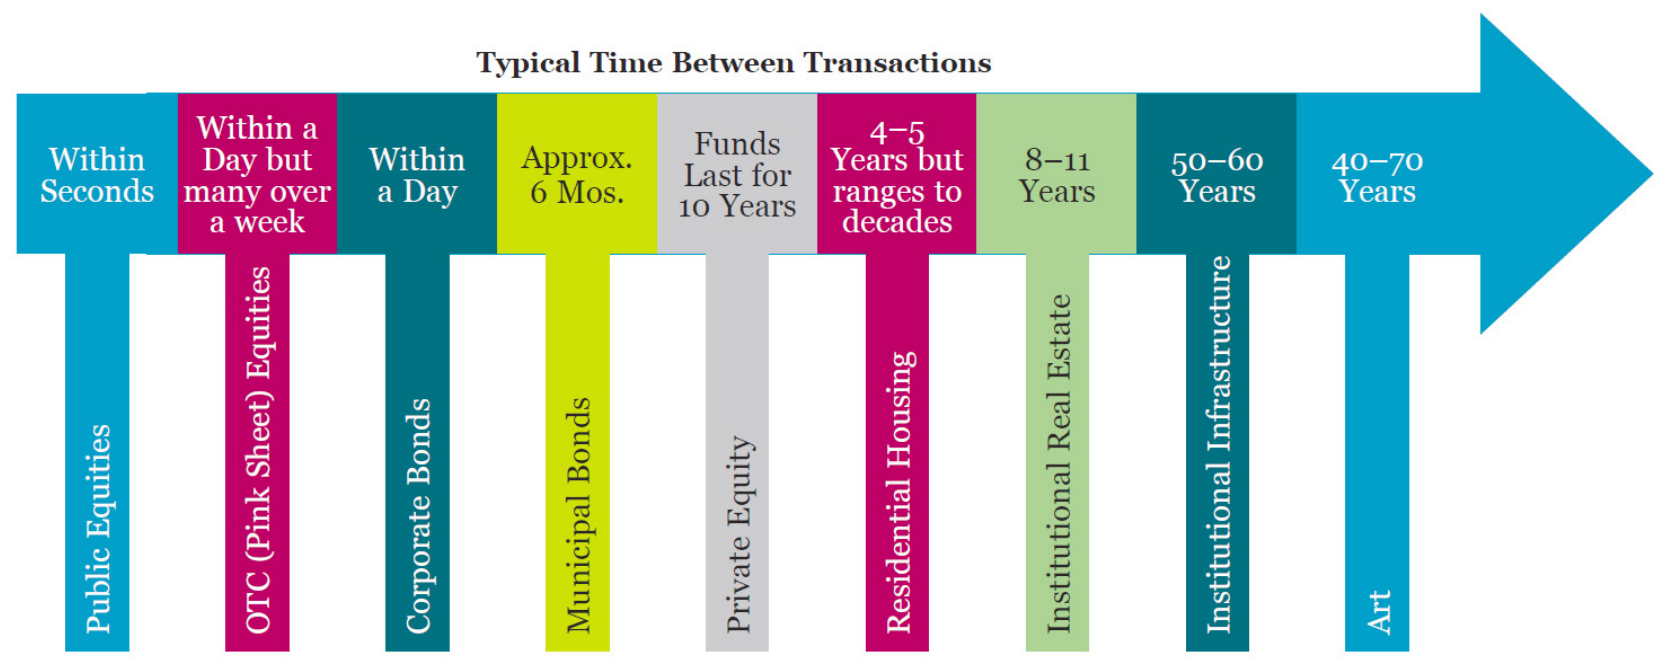
\includegraphics[width=\textwidth]{blackstone.png}
  \caption{Everything Is (Relatively) Liquid\\\textit{Based on \cite{blackstone2015}, source: \cite{ilmanen2011expected}. For illustrative purposes only}}
  \label{fig:blackstone}
\end{figure*}

We see that selling public equities takes several seconds, bonds can be sold within a day, municipal bonds would take weeks or months. Private equities~--- 10 years, real estate~--- 5--10 years, objects of infrastructure such as bridges, roads or factories – tens of years. Works of art may wait for their buyer more than 50 years. 

In this situation, blockchain tokens which can be bought and sold on a decentralized blockchain in less than 10-30 minutes, are an opportunity to tokenize everything that currently takes longer than that to sell. 

The potential tokenization market includes everything that sells over days, weeks or years. Meaning potential for the tokenization market is enormous. The issue currently being addressed by the best blockchains in the world~--- Ethereum and Bitcoin, the issue of having to wait several minutes to receive several transaction confirmations, is no issue to us. 

Asset Tokenization does not work on the market of assets liquid enough to be sold in seconds. The Market Opportunity of BankEx Asset Tokenization stands to the right of Tokens on Figure~\ref{fig:liquidity-over-time}.

\begin{figure*}
  \centering
  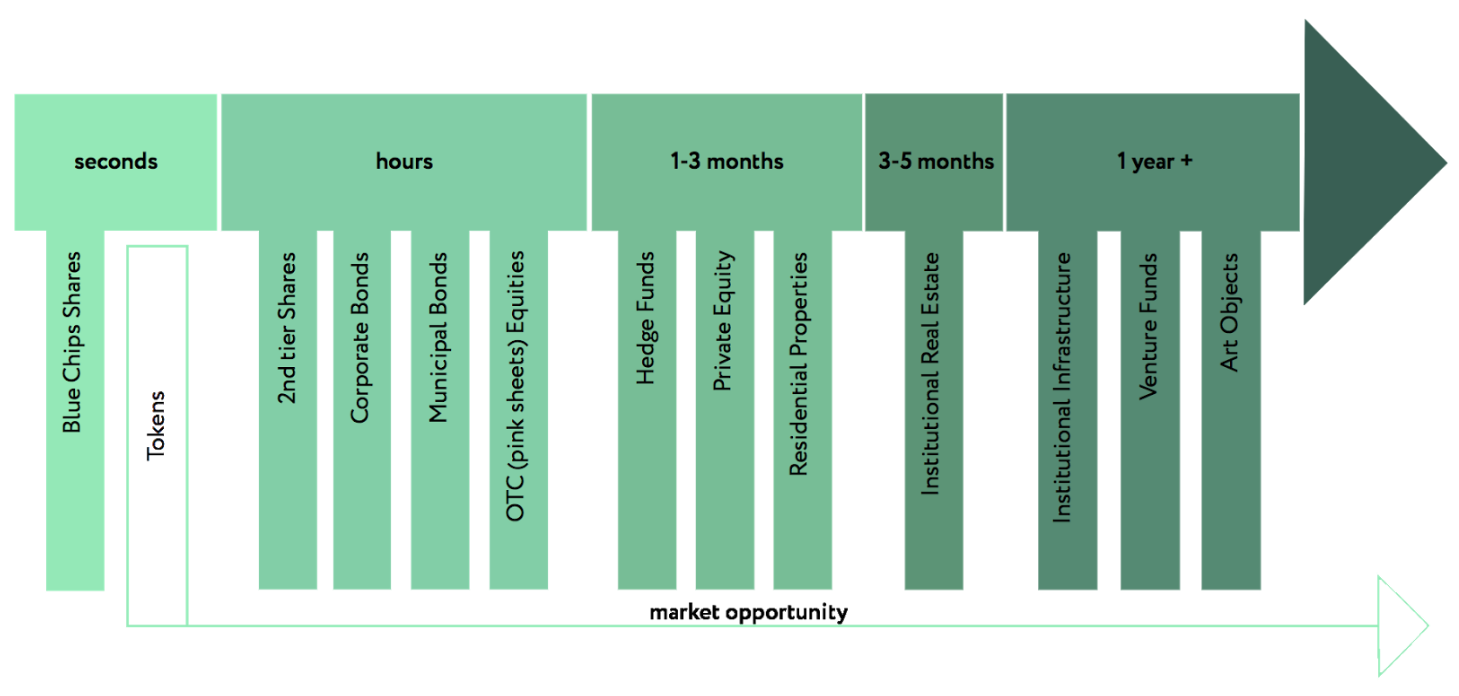
\includegraphics[width=\textwidth]{liquidity-over-time.png}
  \caption{Realizing the Value of Liquid Assets Takes Time}
  \label{fig:liquidity-over-time}
\end{figure*}

We therefore do not compete or fight for the assets that take seconds to sell. This is the market of Ripple\footnote{Ripple provides global financial settlement solutions to enable the world to exchange value like it already exchanges information~--- giving rise to an Internet of Value (IoV). Ripple solutions lower the total cost of settlement by enabling banks to transact directly, instantly and with certainty of settlement. Banks around the world are partnering with Ripple to improve their cross-border payment offerings, and to join the growing, global network of financial institutions and market makers laying the foundation for the Internet of Value. \url{https://ripple.com/xrp/}}~--- the world’s only enterprise blockchain solution for global payments. To them, instantaneous transactions are key, unlike liquidity of Smart Assets during tokenization, where a few seconds don't matter.

In our opinion, target assets for tokenization can include classes of assets with summary capitalization exceeding 100 million USD. 

\subsection{Choosing a Role in New Economy: Coin or Smart Asset}

We receive hundreds of requests: can our business in the real sector be tokenized and how? Many business owners see an opportunity to fund their business using crypto economics via ICO or ITO. Experienced businessmen understand this capital to them is significantly less costly compared to classical sources of capital and is also associated with less administrative risk, as the business decision making center stays in the hands of the owner. In crypto economics there can be no board of directors with members who are non-amicable to you.  

In terms of forming a new economy, BankEx sees a solution to real business funding in separating technological and infrastructure projects from projects in the field of business operating industrial and manufacturing assets. Technological and infrastructure projects that can help decentralized economy develop and become bigger, more convenient, as well as expand usage of technology over the globe can definitely receive funding via ICO. But what about projects in the real economy segment that require tokenization, but lack strong technological teams, experienced IT founders, financial evangelists?

We all know the crowdsale mechanism will only work with influential founders, powerful ideas and a fully transparent vision of the project’s technological realization.  

The answer is obvious: use the technology and infrastructure of core projects in decentralized economy, including ones utilizing an open source protocol. The BankEx Proof-of-Asset Protocol is precisely this kind of solution. 

We present to you the procedure of creating a Smart Asset~--- \textit{ISAO} (\textit{Initial Smart Asset Offering}) based on decentralization protocols, such as the BankEx Proof-of-Asset Protocol. Your asset, even if it’s an offline business, will be able to attract resources by tokenizing its assets using already made powerful technological protocols. You don’t need an ICO procedure, instead you can perform Asset Tokenization of your business using ISAO. 

It’s simple. Use Smart Asset.  

Businesses (farms, stores, manufacturing enterprises) referred to as Smart Assets in our Yellow Paper can be tokenized as part of the ISAO procedure, subsequently forming an \textbf{Asset Community} and receiving returns via Smart Deal.

\subsection{Requirements and Options for Asset Tokenization}

Over the years, working in classic fintech, we have become accustomed to always seek situations that have some sort of problem. Today, we realize that in each of these searches, we would also effectively seek out a problem that prevented an asset from being truly liquid. 

Below are several problems, causing a decrease of an asset’s liquidity, and the more of the below qualities your asset has – the more attractive tokenization of such an asset would be. 

Tokenization of assets gains the greatest value under the following conditions:

\begin{enumerate}[label=(\alph*)]
\item Presence of a large number of asset owners. This means the asset has multiple owners who can have difficulty reaching a consensus. 
\item Distributed asset. You own several office buildings that are rented out several rooms at a time. You can easily see the authenticity of cash flow from the entire asset, but you may find it very difficult, even downright impossible, to figure out the authenticity of cash flow from a single office room. 
\item Standardized end product. This would allow us to identify meta-information when creating a Smart Asset. It’s important for us to be able to bring it to a single basis. 
\item Fungibility (tradability). The possibility of trading one for another. One asset for another asset,  since you as an owner are not concerned with what the asset is. What matters is the cash flow provided by this asset.
\item Use of token as a mean of payment for end-product. An option that would allow the ISAO token released not to be too similar to a payment obligation. A Smart Asset token insures receiving payment, but it can also be used as a means of payment. For example, it can be bought to finance construction of a building, but then this same token can be used to rent a room in this building. As a result, it becomes a utility token, which is important. 
\item Use of the token to own a large asset by a high number of investors and easy means for a buyer to exit co-ownership of a large asset. If an asset can simultaneously be owned by a large number of owners, then it’s makes entry into asset ownership easier. A classical example is shared ownership of large real estate or non-public company shares. Entering such assets with a small share is very complicated at the time.
\item Ability to automatically and unambiguously measure characteristics that directly or indirectly 
indicate a potential quantity and quality of end-products. The ability to integrate regular IoT audit of an asset significantly increases the quality of Smart Asset monitoring. It’s a significant competitive advantage over auditing or rating agencies, whose annual surveys become inferior to real-time IoT audit. 
\item Possibility to withdraw an asset from the owner if the terms of the contract are not fulfilled. This means that, aside from auditing a contract and tokenizing with an escrow module, there is the option of trading the asset, receiving collateral or different contract conditions in the event of a breach of terms. 
\item Control of end-product sales and minimization of the possibility of sales that are not accounted for. This feature does not suit all cases. What this means is that the end product that is tokenized and funded is traced. In the event of tokenizing an agricultural asset such as strawberry, IoT sensors need to be installed that would calculate the number of grown berries to determine whether all of the manufactured berries have brought the appropriate cash flow. These IoT sensors must detect the entire lifetime of an asset up to the generation of cash flow.
\item Assets the transfer of which require high legal and accounting expenditures. Early investors frequently want to sell their assets at the peak of profitability, while other investors are similarly interested in entering ownership of said assets. Tokenization will make such deals significantly simpler and cheaper.
\end{enumerate}

\subsection{Example: Tokenizing Shares in Non-Public Companies}

To give an example of high suitability for tokenization, let us examine late stage private shares that have yet to go public.
These are assets that require very high legal, accounting and administration costs. 

There are many investors in non-public companies who, early ones in particular, are ready to sell their shares, while other investors are interested in entering. But such companies are not public and their shares cannot be traded on the public stock market. Furthermore, they frequently can’t be resold without the approval of company board, since company management must control who their private shareholders are, and prevent their number from exceeding a certain quantity, because otherwise they would breach the limit of investors and become a public company.

These limitations, born from the inefficiency of a historically established system, are an inconvenience to everyone involved~--- both the investors and the company board. In particular, this inefficiency may often lead to disagreements among shareholders and the stalling of company development.

Blockchain technologies allow the necessary details on shares to be recorded in a Smart Contract. Part of the company share, intended for early investors or investors with a miniscule share, is tokenized as an asset in a Smart Asset. Its nominal holder can be any entity permitted by the legislation of the company’s location, such as an SPV. 

After that, from the nominal token-holder’s perspective, they can easily change upon reaching consensus among themselves, as buyers or sellers of tokens of this Smart Asset. At the same time, shareholders are essentially not changing. All presence rights of token holders are passed to the SPV. For non-public companies that don’t want changes in their board of governing shareholders, obtaining liquidity of their capital via tokenization of part of their equity into a Smart Asset is essentially the only mutually acceptable option for all sides involved. 
For early investors this method of investment becomes a new step to decreasing investment risks, and as a result increases the possibility of investment into formerly unavailable assets.

\section{Fundamental Advantage of Tokenization for an Asset}

The analytical block of BankEx, gathering and analyzing financial technologies from all over the world for several years, is seeing an interesting trend that has been forming around financial tools during the last few years. 

If we take apart the basic needs of a person or a company in terms of movement of funds, it would be easy to discover that every person or company does not have that many basic financial needs, namely:
    
\begin{itemize}
\item spending money;
\item moving money;
\item storing money;
\item earning money.
\end{itemize}

By correlating these basic financial needs with the current range of financial technologies it turns out that today there is a strong leaning towards saturation of certain needs with financial technologies:

\begin{itemize}
\item \textbf{spending money}~--- the need that is most saturated and easiest to digitize. There are currently thousands of companies that help a person or a company to easily and quickly spend their money;
\item \textbf{moving money}~--- similar in terms of saturation, but this basic need has several unresolved issues, including ones currently being addressed by our colleagues at Ripple;
\item \textbf{storing money}~--- the need for people and companies to keep their money in their pockets is virtually non-existent today, having fully been digitized and moved to plastic cards and a whole range of innovative solutions. 
\end{itemize}

The BankEx Proof-of-Asset Protocol allows people and organizations to fulfill an important, vital need~--- the need to earn money. By becoming part of the Asset Community you will have the option of earning, and thus realizing yourself in fields of your choosing. 

Cryptocurrencies solve the global issue of digitization of the human need to earn money, and altogether the emergence of cryptocurrencies is a technological response, solving this fundamental issue. 

SmartDeal based on open source Smart Asset by the Proof-of-Asset Protocol is the next step. You will be able to build your future with your own hands.

\section{BankEx Ecosystem}

\textit{In progress...}

\section{Protocol Description}

\textit{In progress...}

\section{Proof-of-Asset Protocol Implementation on Ethereum Platform}

\subsection{Blockchain-agnostic}

\textit{In progress...}

\subsection{BKX Tokens}

\textbf{Value}. The smallest subdenomination of BKX is called Cent. All integer values are counted in Cent in the BankEx ecosystem. BKX denomination is defined in Table~\ref{tab:tokens}.

\begin{table*}
    \caption{BKX Token Denomination}
    \label{tab:tokens}\centering
    \begin{tabularx}{0.5\textwidth}{|X|X|}
        \hline
            \thead{Multiplier} & \thead{Name} \\
        \hline
            \makecell{$10^0$} & \makecell{BKX Cent} \\
            \makecell{$10^2$} & \makecell{BKX} \\
        \hline
    \end{tabularx}
\end{table*}

\textbf{Transaction} is a single cryptographically signed transaction based on the Ethereum blockchain. We have two types of transactions: \textit{smart-asset creation} and \textit{asset transfer} (from one wallet to another one, from a wallet to the BankEx Exchange and vice-versa). Each smart-asset will come with an internal reserve of BKX that will be used by all the functions used by the smart asset in the BankEx ecosystem. Functions associated with a transaction:

\begin{description}
\item[nonce]--- scalar value representing number of transactions sent by the sender, $T_{number}$
\item[BankEx gas price]--- scalar value representing the number of BKX~Cent used to pay for the all computational costs included by the transaction accomplishment, $T_{BKX_{gas}}$
\item[BankEx gas limit]--- maximal value of gas that be used to execute a transaction, $T_{BKX_{gasLimit}}$
\item[to]--- address of the recipient. It will be represented in 160-bit similar to the Ethereum one, $T_{to}$
\item[value]--- scalar value that represents a quantity of a given type of smart-asset, $T_{value}$
\item[init]--- an unlimited size byte array representing the EVM-code for account initialization procedure, same as in Ethereum, used when smart asset is created, $T_{init}$
\item[data]--- unlimited size byte array representing input data of a message call transaction, similar to Ethereum, $T_{data}$
\end{description}

This way any operations with a given smart asset can be represented by:

\begin{equation}
    \Omega(T) \equiv
    \begin{cases} 
        (T_{number}, T_{BKX_{gas}}, \\T_{BKX_{gasLimit}}, T_{to}, \\T_{value}, T_{init}) & \text{if } T_{to} = \emptyset, \\
        \\
        (T_{number}, T_{BKX_{gas}}, \\T_{BKX_{gasLimit}}, T_{to}, \\T_{value}, T_{data}) & \text{otherwise}
    \end{cases}
\end{equation}

Block and World State \cite{wood2014ethereum} structures will be similar to Ethereum ones, since BankEx ecosystem will be based on the Ethereum blockchain.

\textbf{Smart asset creation}. This operation involves a few parameters: sender ($s$), original transactor ($ot$), available BKX gas ($g_{BKX}$), BKX gas price ($p_{BKX}$), BankEx escrow ($b_{escrow}$) and endowment ($\nu$) with the arbitrary length byte array ($i$), $EVM$ code and the depth of the message call/smart assert creation stack ($e$) (the parameters $s$, $ot$, $\nu$, $i$, $EVM$ and $e$)are identical to ones encoded in the Ethereum token.

The first step of the smart asset creation will always involve the creation of a token on the Ethereum blockchain. We use the name $\sigma$ as in our Ethereum token that precedes the smart asset.

We formally describe the creation of smart asset by:

\begin{equation}
    \left(\sigma', g', A\right) \equiv \Lambda_2\left(\sigma, s, ot, g_{BKX}, p_{BKX}, b_{escrow}, \nu, i, e\right)
\end{equation}

\subsection{Token Economics}

\subsubsection{BKX Token Circulation in BankEx Ecosystem}

\textit{In progress...}

\subsubsection{Transaction Types in BankEx Ecosystem and Value Calculation Formulas}

In cases when it's possible to use both BKX gas and Ethereum it will be cheaper to use BKX creating additional stimules to use them.

\begin{equation}
	\begin{split}
    	f_{totalGas} & = \delta_{SA_{Creation}} \times f_{SA_{Creation}} \\
    	& + \delta_{Transfer_{Internal}} \times f_{Transfer_{Internal}} \\
    	& + \delta_{Withdrawal} \times f_{Withdrawal} \\
    	& + \delta_{Oracle} \times f_{Oracle} \\
    	& + \delta_{Market} \times f_{Market}
    \end{split}
\end{equation}

\begin{equation*}
	\text{where } \delta_i = 
	\begin{cases}
		1 & \text{if \textit{service is requested}} \\
		0 & \text{otherwise}
	\end{cases}
\end{equation*}

\textbf{Execution of smart-asset transaction}. Every operation involving smart assets will be using BankEx gas. We have developed system of fees, described in Table~\ref{tab:op-fees}.

\begin{table*}
    \caption{System operation fees}
    \label{tab:op-fees}\centering
    \begin{tabularx}{0.85\textwidth}{|c|c|X|}
		\hline
			\thead{Purpose} & \thead{BKX \\ Amount \\ used} & \thead{Details} \\
	    \hline
    		\makecell[l]{Creation of a Smart Asset} & \makecell{100 =<} & \makecell[l]{Amount depends on the complexity of the \\ Smart Asset and Ethereum Network load} \\
		\hline
            \makecell[l]{Transfer of the Smart Asset \\in BankEx ecosystem} & \makecell{2 =<} & \makecell[l]{Amount depends on the complexity of the \\ Smart Asset and Ethereum Network load} \\
		\hline
            \makecell[l]{Destruction of the Smart Asset} & \makecell{5 =<} & \makecell[l]{Amount depends on \\ the Ethereum Network load} \\
		\hline
            \makecell[l]{Adding a step in the originator \\ verification chain} & \makecell{150 =<} & \makecell[l]{Depends on the service which will \\ be requested (scoring, KYC\ldots)} \\
		\hline
            \makecell[l]{Requesting the \enquote{Verified Status} \\ for the Smart Asset} & \makecell{400 =<} & \makecell[l]{Depends on the type \\and complexity of the asset} \\
		\hline
            \makecell[l]{Requesting Escrow Services} & \makecell{50 =<} & \makecell[l]{Depends on the type} \\
	    \hline
    \end{tabularx}
\end{table*}

\subsubsection{BKX Circulation in BankEx Ecosystem}

\textit{In progress...}

\subsubsection{Microsoft Azure Cloud Infrastructure Usage for Storage of Asset's Extra Data}

\textit{In progress...}

\end{multicols}

\newpage
\appendix

\section{Terminology}
\begin{description}
\item[Blockchain]~--- is a continuously growing list of records, called \textit{blocks}, which are linked and secured using cryptography \cite{bitcoinComprehensive2016}, \cite{wikipediaBlockchain}.
\item[ISAO]~--- Initial Smart Asset Offering
\item[Tokenization]~--- process of converting rights into digital token to be circulated over blockchain with low transactional fees. Tokenization is a blockchain equivalent of securitization.
\end{description}

\printbibliography

\end{document}
